\documentclass[12pt]{article}
\usepackage[margin=0.75in]{geometry}
\usepackage{graphicx}
\usepackage{float}
\setlength{\parindent}{0mm}

\begin{document}

{\centering
\large Physics I: Lab 06 \par
\large Work and Power \par
}
\hfill \break \vspace{-4mm}

\underline{\textbf{Part 1}} \par
Use a constant horizontal force to push a block ($v_i = 0$) up a ramp that has friction.
Choose and record all relevant values.
Identify all forces present, label each one as conservative or non-conservative, and calculate the amount of work each one does on the block.
Use these work values to calculate the expected final velocity after some time interval.
Compare this calculation to the final velocity measured by IP.

%
\begin{figure}[H]
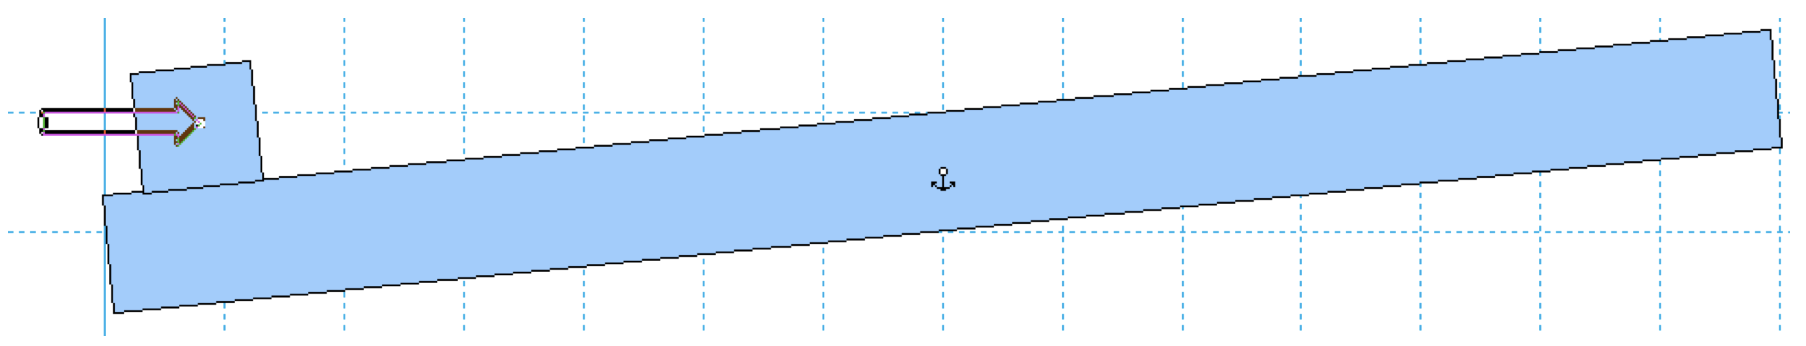
\includegraphics[scale=0.50]{figures/fig1.png}
\end{figure}
%

\underline{\textbf{Part 2}} \par

In this part you will measure your maximum power by jumping as high as you can.
\begin{itemize}
\item Use a meter stick to measure the three relevant heights shown in the figure (with uncertainty).
\item Also write down your weight (converted to kg, with uncertainty).
\item Assume constant acceleration and force, and use kinematics to calculate relevant velocities and time intervals. Also calulate the uncertainty in these quantities using error propagation.
\item Finally, calculate your power during the jump with uncertainty. Record your result in Watts and horsepower.
\end{itemize}

%
\begin{figure}[H]
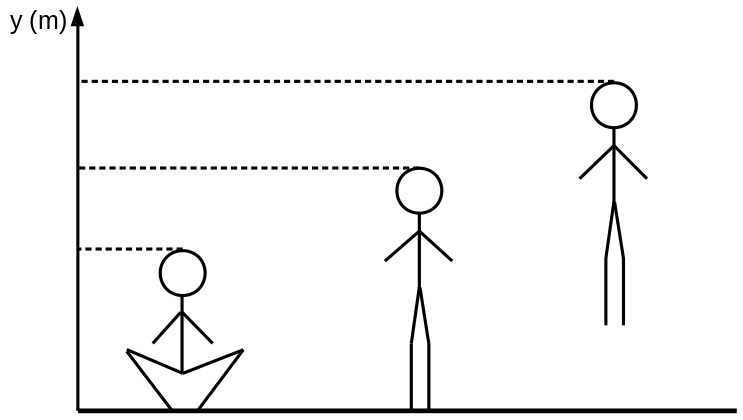
\includegraphics[scale=0.50]{figures/fig2.png}
\end{figure}
%

\end{document}
